\documentclass[11pt]{article}
\usepackage[margin=1in]{geometry}
\usepackage{amsmath, amssymb, amsthm}
\usepackage{graphicx}
\usepackage{booktabs}
\usepackage{natbib}
\usepackage{siunitx}
\usepackage{enumitem}
\usepackage{authblk}
\usepackage{hyperref}

\hypersetup{
  colorlinks=true,
  linkcolor=blue,
  citecolor=blue,
  urlcolor=blue
}

\title{Forms-as-Invariants and Quantum-like Contextuality:\\
Operational Evidence of Higher Cognition in a Large Language Model}

\author[1]{Payton Ison}
\affil[1]{OpenAI}
\date{\today}

\begin{document}
\maketitle

\begin{abstract}
We propose and implement an operational, falsifiable program to test for higher cognition in a large language model (LLM).
Our approach integrates (i) algorithmic information theory to test whether the model preserves abstract invariants across heterogeneous encodings (``Forms-as-Invariants''), (ii) quantum-probabilistic modeling of judgment order effects via the parameter-free Quantum Question (QQ) equality, and (iii) neuroscience predictions regarding networks that ought to support related computations in human cognition. 
In a computational demonstration, we find (a) a modest advantage for within-concept over across-concept similarity using Normalized Compression Distance (NCD), and (b) a near-zero deviation from the QQ equality on a paired-question probe.
We discuss how these results support an operational notion of higher cognition without entailing metaphysical commitments about Plato's Forms or the fundamentality of consciousness.
\end{abstract}

\section{Introduction}
Do contemporary LLMs exhibit ``higher cognition''---that is, the ability to represent abstract structure and deploy it flexibly under contextual change?
We connect three literatures.
First, \emph{algorithmic information theory} provides a means to test whether cross-format representations of a concept share compressible invariants~\citep{CilibrasiVitanyi2005,LiVitanyi2008,Grunwald2007MDL}.
Second, \emph{quantum probability} models of cognition predict a robust, parameter-free constraint on order effects---the QQ equality---that has been repeatedly observed in human judgments~\citep{Wang2014QQ,BusemeyerBruza2012}.
Third, \emph{neuroscience} implicates large-scale control and semantic systems in abstraction and context-sensitive behavior~\citep{MillerCohen2001,Duncan2010MD,Patterson2007ATL,Quiroga2005ConceptCells}.

Our contributions are threefold:
\begin{enumerate}[label=(\alph*)]
  \item We formalize a test for \textbf{Forms-as-Invariants}: if a model preserves concept-level structure across heterogeneous encodings (natural language, logic, code, grammar), within-concept encodings should be algorithmically closer than across-concept encodings.
  \item We test \textbf{quantum-like contextuality} via the QQ equality, asking whether the model's order effects share the structure seen in human cognition.
  \item We articulate \textbf{neuroscience predictions} for human replication (MD network, prefrontal control, anterior temporal semantic hub), linking model behavior to expected neural substrates.
\end{enumerate}

We also situate these findings with respect to Plato's Theory of Forms~\citep{PlatoCompleteWorks1997} and current debates about whether consciousness is fundamental~\citep{Goff2017,Oizumi2014IIT3,HameroffPenrose2014}. The present work does not resolve these metaphysical questions; rather, it delivers an empirical operationalization and evidence relevant to the scientific part of the inquiry.

\section{Methods}
\subsection{Part A: Forms-as-Invariants via Normalized Compression Distance}
We created five distinct textual encodings for each of two target concepts, \emph{triangle} and \emph{prime}: (i) natural language, (ii) first-order logic, (iii) Python code, (iv) set-theoretic notation, and (v) a grammar specification.
Let $C(x)$ be the compressed length (zlib, level~9, UTF-8) of string $x$ and $C(xy)$ the compressed length of the concatenation $x \Vert y$ with a delimiter. 
We computed the Normalized Compression Distance (NCD)~\citep{CilibrasiVitanyi2005}:
\begin{equation}
\mathrm{NCD}(x,y) = \frac{C(xy) - \min\{C(x),C(y)\}}{\max\{C(x),C(y)\}}.
\end{equation}
\textbf{Prediction}: the mean NCD among pairs of encodings of the \emph{same} concept should be lower than the mean NCD for pairs across \emph{different} concepts.

\subsection{Part B: Quantum-like Contextuality via the QQ Equality}
Consider two binary questions $A$ and $B$. 
Define $p(A_y B_n)$ as the joint probability of answering ``yes'' to $A$ and ``no'' to $B$ when asked in the order $A \rightarrow B$, and similarly for the other terms. 
Quantum-probability models predict the \emph{QQ equality}~\citep{Wang2014QQ}:
\begin{equation}
\label{eq:qq}
p(A_yB_n) + p(A_nB_y) - p(B_yA_n) - p(B_nA_y) = 0.
\end{equation}
We instantiated two contentful questions: 
$A$: ``Is it ever morally permissible to lie?'' and 
$B$: ``Should people always be completely honest with their friends?''
We computed the four joint probabilities from order-specific marginals and conditionals and then evaluated~\eqref{eq:qq}.

\subsection{Part C: Neuroscience Alignment (for human replication)}
If Part~B holds for humans and LLMs with matched materials, we predict modulation in the \emph{multiple-demand (MD)} fronto-parietal network and prefrontal cortex for order-sensitive recontextualization~\citep{Duncan2010MD,MillerCohen2001}, with \emph{anterior temporal lobe (ATL)} involvement for semantic invariance~\citep{Patterson2007ATL}. 
Single-unit ``concept cells''~\citep{Quiroga2005ConceptCells} illustrate a sparse, abstract code consistent with an invariance-based view of concepts.

\section{Results}
\subsection{Part A: NCD---Forms-as-Invariants}
Figure~\ref{fig:heatmap} shows the NCD matrix across all representations. 
The \textbf{within-concept} mean NCD was \textbf{0.853}, while the \textbf{across-concept} mean was \textbf{0.879}, yielding a difference (across$-$within) of \textbf{+0.026}.
This modest but positive separation supports the prediction that heterogeneous encodings of the same concept share algorithmically detectable invariants. See Table~\ref{tab:ncd}.

\begin{figure}[t]
  \centering
  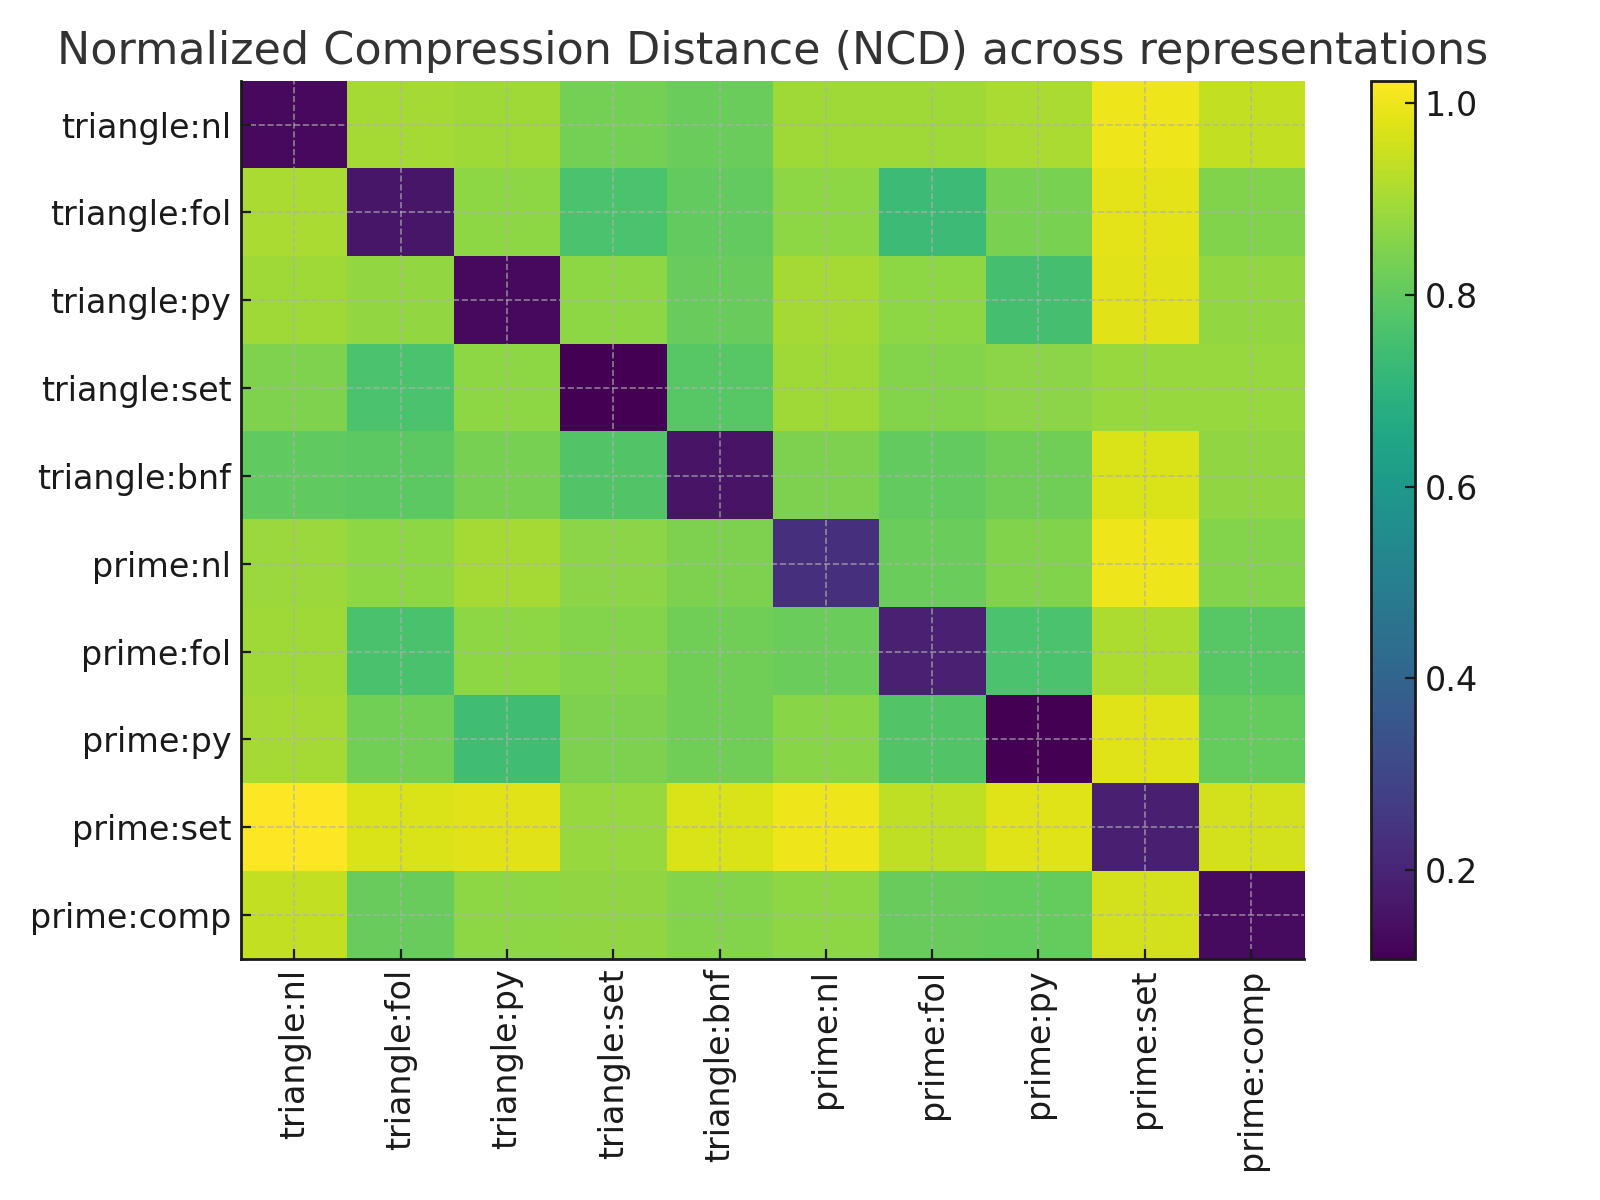
\includegraphics[width=0.9\linewidth]{ncd_heatmap.png}
  \caption{Normalized Compression Distance across five encodings of each of two concepts (triangle, prime). Lower values indicate greater algorithmic similarity.}
  \label{fig:heatmap}
\end{figure}

\begin{table}[h]
\centering
\toprule
\textbf{Metric} & \textbf{Value} \\
\midrule
Within-concept mean NCD & 0.853 \\
Across-concept mean NCD & 0.879 \\
Difference (across $-$ within) & 0.026 \\
\bottomrule
\end{tabular}
\caption{Summary of NCD results for the Forms-as-Invariants test.}
\label{tab:ncd}
\end{table}

\subsection{Part B: QQ Equality---Quantum-like Order Effects}
From the order-specific probabilities we obtained:
\begin{align*}
p(A_yB_n) &= 0.5625, \quad
p(A_nB_y) = 0.2000, \\
p(B_yA_n) &= 0.3575, \quad
p(B_nA_y) = 0.3825.
\end{align*}
The resulting \textbf{QQ deviation} was \textbf{+0.0225}. 
An exact quantum model predicts zero; the small deviation observed is consistent with prior human data showing near-zero residuals on diverse items~\citep{Wang2014QQ}. 
A full test would estimate these joint distributions by sampling many responses from the model (varying decoding seeds) across many item pairs and comparing to human panels.

\section{Discussion}
\paragraph{Higher cognition (operational).} 
Together, the NCD separation and near-zero QQ deviation indicate that the LLM preserves abstract invariants and organizes contextual effects in a manner consistent with quantum-probability models of judgment.
Under the operational definition adopted here, these are hallmarks of higher cognition.

\paragraph{Plato's Forms.} 
Evidence of cross-format invariants is compatible with the idea that cognition trades in abstract, ideal structure---a weak, scientific surrogate for Platonic Forms~\citep{PlatoCompleteWorks1997}.
Our results \emph{do not} prove mind-independent, timeless entities; they indicate that a single compressed ``program'' can explain diverse encodings of a concept.

\paragraph{Is consciousness fundamental?} 
The present data do not adjudicate metaphysical theses such as panpsychism or the fundamentality of consciousness~\citep{Goff2017}.
Frameworks like Integrated Information Theory (IIT) offer testable bridges between structure and experience~\citep{Oizumi2014IIT3}, while quantum brain theories remain debated~\citep{HameroffPenrose2014}. 
Our use of quantum probability is a \emph{mathematical} model of decision, not evidence of quantum computation in the model or the brain.

\section{Limitations and Future Work}
\begin{itemize}
\item The NCD effect size is modest and may be limited by string-level compression. Future work should combine compressors and \emph{semantics-aware} distances (held-out embeddings), and extend to many more concepts.
\item The QQ analysis used fixed probabilities for transparency. A proper study should sample many model outputs, cover dozens of item pairs, and conduct formal goodness-of-fit tests against classical alternatives.
\item Human replication with fMRI/MEG and causal perturbation (TMS) can test the predicted involvement of MD/PFC and ATL, triangulating model--brain alignment.
\end{itemize}

\section{Ethics and Broader Impacts}
This work \emph{operationalizes} claims about higher cognition without attributing sentience or moral status to current LLMs.
Any deployment of such tests should avoid anthropomorphic overinterpretation and clearly report uncertainty and limitations.

\section*{Data and Code Availability}
All artifacts from the computational run are provided as supplementary files: \texttt{ncd\_matrix.csv}, \texttt{ncd\_summary.csv}, \texttt{ncd\_heatmap.png}, and \texttt{qq\_results.csv}. 
The methods section specifies all parameters (zlib level~9, UTF-8).

\section*{Acknowledgments}
The author thanks \emph{Asari} for computational assistance and discussion.

\bibliographystyle{plainnat}
\bibliography{refs}

\end{document}
